\documentclass[12pt]{article} % 12 -- размер шрифта
\usepackage{cmap} % Чтобы можно было копировать русский текст из pdf
\usepackage[T2A]{fontenc}
\usepackage[russian]{babel} % В частности эта строка отвечает за правильные переносы слов в конце строки
\usepackage[utf8]{inputenc} % Проверьте, что кодировка файла -- тоже utf8
\usepackage{amsmath, amssymb} % Чтобы юзать математические символы
\usepackage{ dsfont }
\usepackage{ wasysym }
\usepackage[makeroom]{cancel}
\usepackage{listings}
\usepackage{tcolorbox}

\usepackage[utf8]{inputenc}

\usepackage{listings}
\usepackage{xcolor}
\usepackage{tikz}
\usetikzlibrary {positioning}

\newcommand \tab[1][1cm]{\hspace*{#1}}

\definecolor{codegreen}{rgb}{0,0.6,0}
\definecolor{codegray}{rgb}{0.5,0.5,0.5}
\definecolor{codepurple}{rgb}{0.58,0,0.82}
\definecolor{codepink}{rgb}{0.92,0.01,0.55}
\definecolor{backcolour}{rgb}{0.95,0.95,0.92}

\lstdefinestyle{mystyle}{
	backgroundcolor=\color{backcolour},   
	commentstyle=\color{codegreen},
	keywordstyle=\color{magenta},
	numberstyle=\tiny\color{codegray},
	stringstyle=\color{codepurple},
	basicstyle=\ttfamily\footnotesize,
	breakatwhitespace=false,         
	breaklines=true,                 
	captionpos=b,                    
	keepspaces=true,                 
	numbers=left,                    
	numbersep=5pt,                  
	showspaces=false,                
	showstringspaces=false,
	showtabs=false,                  
	tabsize=2
}

\lstset{style=mystyle}

\begin{document}

\title{Алгоритм Евклида}
\author{Парамонов Антон Игоревич}
\date{}
\maketitle
\section{Наибольший общий делитель}
\begin{tcolorbox}[colback=white, colframe=black]
	\textit{Определение:}\\
	Наибольший общий делитель (НОД) двух целых чисел $a$ и $b$ - это наибольшее натуральное число, на которое делится и $a$, и $b$.\\
	Например, $\mathrm{\text{НОД}}(30, 24) = 6$, а $\mathrm{\text{НОД}}(30, 23) = 1$.
\end{tcolorbox}
О НОД-е можно думать с алгебраической стороны, а именно, что НОД$(a, b) = d$ тогда и только тогда, когда $a = c_1\cdot d,\ b = c_2\cdot d$, где $c_1$ и $c_2$ какие-то взаимнопростые (не имеют общих делителей кроме 1) числа. Действительно, не вызывает сомнений то, что $a\ \vdots\ d$ и $b\ \vdots\ d$, т.е. $d$ - общий делитель. То, что он наибольший, следует из взаимной простоты $c_1$ и $c_2$. Действительно, предположим, что $d$ - не наибольший, т.е. есть некое число $d'$, такое что $a\ \vdots\ d'$, $b\ \vdots\ d'$, $d' > d$. Рассмотрим дробь $\frac{d}{d'}$. Она $ < 1$, т.к. $d < d'$. Значит, когда мы максимально сократим ее, она примет вид $\frac{k}{l}$, где $l > 1$. Мы знаем, что $a\ \vdots\ d' \Leftrightarrow \dfrac{c_1 \cdot d}{d'}$ - целое число $\Leftrightarrow \dfrac{c_1 \cdot k}{l}$ - целое число $\Leftrightarrow c_1 \cdot k\ \vdots\ l \Leftrightarrow c_1\ \vdots\ l$, т.к. $k$ и $l$ взаимнопросты. Аналогично $c_2\ \vdots\ l$. Но $c_1$ и $c_2$ взаимнопросты, а $l > 1$. Противоречие.
\newpage

Можно представлять НОД и графически, с помощью кругов Эйлера.\\
\\
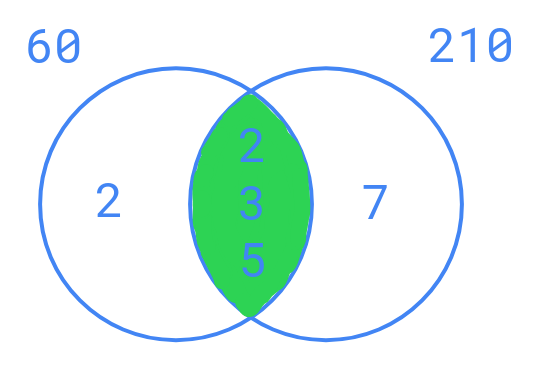
\includegraphics[scale=0.6]{gcd.png}\\
\\
Здесь в круге для каждого числа (60ти и 210ти) написаны его простые делители. Делители $2, 3, 5$ - общие, поэтому НОД(60, 210) = $2\cdot3\cdot5 = 30$.\\
\section{Алгоритм Евклида}
Алгоритм Евклида - быстрый алгоритм для нахождения наибольшего общего делителя двух чисел. Он был придуман греческим математиком Евклидом еще в 3ем веке до нашей эры.
\subsection{Идея}
Алгоритм этот рекурсивный. Как мы помним, основная идея рекурсии состоит в том, чтобы свести имеющуюся задачу к такой же, но попроще.\\
Пусть нам нужно посчитать НОД чисел a и b. Предположим, не умаляя общности, что $a > b$. Мы знаем, что $a$ и $b$ представляются в виде $a = c_1 \cdot d$, $b = c_2 \cdot d$, но что это за $c_1, c_2$ и $d$, конечно, не знаем и хотим узнать $d$. Заметим теперь, что если два числа делились на $d$, то и их разность будет делиться на $d$. Действительно, $a - b = c_1\cdot d - c_2 \cdot d = d(c_1 - c_2)\ \vdots\ d$. Притом утверждается, что НОД($b$, $a - b$) = $d$. И правда, как мы только что показали $d$ - их общий делитель, докажем, что он наибольший. Предположим противное. Пусть есть $d'$, такой что $b\ \vdots\ d'$, $a - b\ \vdots\ d'$, $d' > d$. Поскольку $b\ \vdots\ d'$ и $a - b\ \vdots\ d'$, заключаем, что $(a - b) + b = a\ \vdots\ d'$. Но тогда НОД($a$, $b$) $\geq d' > d$, противоречие.

Таким образом мы показали, что НОД($a$, $b$) = НОД($a - b$, $b$), т.е. мы упростили себе задачу, уменьшив одно из чисел!
\subsubsection{Когда заканчивать}
В рекурсии мы упрощаем себе задачу до тех пор, пока ответ не станет очевидным. В каком случае мы можем назвать ответ сразу? Например, когда нас просят посчитать НОД двух одинаковых чисел: \\
НОД($a$, $a$) $= a$\\
или когда одно из чисел равно 0: \\
НОД($0$, $a$) $=$ НОД($a$, $0$) $= a$\\
Мы будем использовать именно второй вариант.
\subsection{Пример}
Рассмотрим пример. Пусть нам нужно посчитать НОД 33 и 6. \\
НОД(33, 6) = НОД(27, 6) = НОД(21, 6) = НОД(15, 6) = НОД(9, 6) = НОД(3, 6) = НОД(3, 3) = НОД(3, 0) = 3.\\
\subsection{Ускоряемся}
Пример сработал, но видно, что мы слишком долго отнимали 6ки из 33ех. Заметим, что мы отнимали 6ки до тех пор, пока не уменьшились до числа меньшего 6ти. Иначе говоря мы получали такое $r$, что $33  \underbrace{- 6 - 6- \ldots -6}_{k} = r$, $r < 6$. Или $33 = 6\cdot k + r$. Так что же такое $r$? Правильно, остаток при делении на 6! Т.е. мы могли не вычитать 6ки, а сразу заменить $33 \rightarrow 33\ \%\ 6$.\\
Говоря в общем, мы поняли, что НОД($a$, $b$) $=$ НОД($a\ \%\ b$, $b$). 
\newpage
\subsection{Код}
Реализация на \textit{Python3}
\begin{lstlisting}[language=Python]
def gcd(a, b):  # Greatest Common Divisor
	mn = min(a, b)
	mx = max(a, b)
	if mn == 0:
		return mx
	return gcd(mx % mn, mn)
\end{lstlisting}
Поскольку нам важно, кто из чисел $a$ и $b$ больше, во 2ой и 3ей строчках заведем переменные, соответствующие меньшему и большему из них. (Переменные называются именно \colorbox{backcolour}{mn, mx}, чтоб не путаться с названиями встроенных функций \colorbox{backcolour}{\textcolor{codepink}{min}} и \colorbox{backcolour}{\textcolor{codepink}{max}}).\\
В 6ой строчке происходит рекурсивный вызов функции \colorbox{backcolour}{gcd} для более простой задачи (уменьшенных чисел), она возвращает ответ, а мы знаем, что ответ у упрощенной задачи такой же, как у нашей, так что и сами возвращаем его.\\
Можно привести следующее сравнение. Представьте, что мама попросила вас сходить в магазин за молоком. А вы, в свою очередь, попросили об этом младшего брата. Младший брат принес вам молоко, а вы отдали его маме.
\section{Наименьшее общее кратное}
\begin{tcolorbox}[colback=white, colframe=black]
	\textit{Определение:}\\
	Наименьшее общее кратное (НОК) двух натуральных чисел $a$ и $b$ - наименьшее натуральное число, такое что оно делится и на $a$, и на $b$.\\
	Например, $\mathrm{\text{НОК}}(12, 8) = 24$, а $\mathrm{\text{НОК}}(5, 7) = 35$.
\end{tcolorbox}
\newpage
Наименьшее общее кратное $a$ и $b$ - это число, которое включает в себя минимальное количество простых чисел, таких чтоб среди них содержались все простые делители (с учетом кратности) $a$ и $b$. С точки зрения кругов Эйлера, нужно брать объединение двух кругов.\\
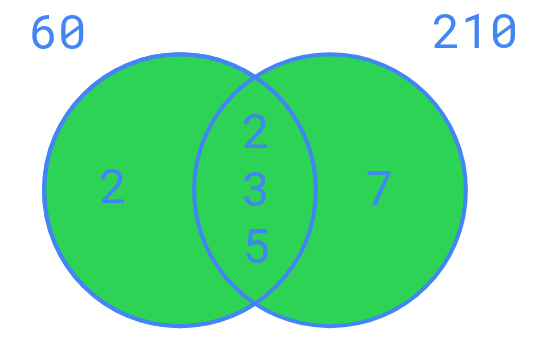
\includegraphics[scale=0.7]{lcm.png}\\
Можно подумать, что этого объединения можно достичь, перемножив числа, однако это не совсем верно, т.к. в таком случае мы дважды учтем то, что находится в пересечении, т.е. НОД. Поэтому, после перемножения нужно убрать его, т.е. поделить.\\
И того: НОК($a$, $b$) = $\frac{a\cdot b}{\text{НОД}(a, b)}$
\end{document}